\documentclass[11pt,fleqn]{article}

\setlength {\topmargin} {-.15in}
\setlength {\textheight} {8.6in}

\usepackage{amsmath}
\usepackage{amssymb}
\usepackage{color}
\usepackage{tikz}
\usetikzlibrary{automata,positioning,arrows}
\usepackage{diagbox}
\usepackage{stackrel}
\begin{document}


\textbf{Exercise 1.4.10:} Modify binary search so that it always returns the element with the smallest
index that matches the search element (and still guarantees $logarithmic$ running time).\\

\textbf{Solution:} Recall Binary search works by picking a midpoint value and then recursively checking each half(left or right) depending on the key we are looking for. RHS are elements that are larger than the key while LHS are elements that are smaller than the key. Binary Search only works for sorted arrays. To solve the above problem, continue binary search on LHS until that number is the last instance. Eliminate RHS each time since that half consists of keys that are larger.\\

Another solution would be to check left side of array until you find last instance. However, this becomes $O(N)$ runtime and we want $O(nlogn)$.

\begin{center}
	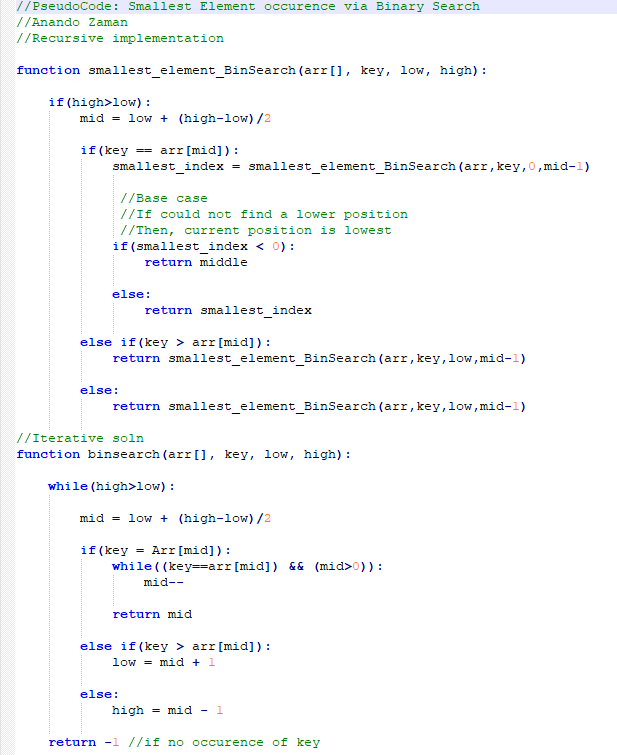
\includegraphics[scale = 1]{1.4.10.png}
	\end{center}

\end{document}
